
%(BEGIN_QUESTION)
% Copyright 2009, Tony R. Kuphaldt, released under the Creative Commons Attribution License (v 1.0)
% This means you may do almost anything with this work of mine, so long as you give me proper credit

A gas enclosed inside a chamber may act as a primitive thermometer, based on the {\it Ideal Gas Law}:

$$PV = nRT$$

\noindent
Where,

$P$ = Absolute pressure (atmospheres)

$V$ = Volume (liters)

$n$ = Gas quantity (moles)

$R$ = Universal gas constant (0.0821 L $\cdot$ atm / mol $\cdot$ K)

$T$ = Absolute temperature (K)

\vskip 10pt

Suppose a hollow metal chamber filled with air connects to a pressure gauge through a capillary tube (a tube with a very small internal diameter).  As the chamber heats and cools, the air pressure inside changes as well:

$$\includegraphics[width=15.5cm]{i04013x01.eps}$$

At room temperature (20 $^{o}$C), the chamber's air pressure is 1 atmosphere.  How high would the chamber's temperature have to be raised in order to increase the internal air pressure to 2 atmospheres?  Supposing the pressure gauge is calibrated to read in units of PSIG, how high would it register at this temperature?

What class of filled-bulb temperature instrument does this arrangement represent?  Class I?  Class II?  Class III?  Class V?

\vskip 20pt \vbox{\hrule \hbox{\strut \vrule{} {\bf Suggestions for Socratic discussion} \vrule} \hrule}

\begin{itemize}
\item{} Describe the effect of a tiny {\it leak} in this filled-bulb system.
\item{} How should an instrument technician calibrate a filled-bulb temperature sensor?  You certainly cannot connect a millivoltage or resistance source to the instrument as you can with thermocouple and RTD instruments!
\end{itemize}

\underbar{file i04013}
%(END_QUESTION)





%(BEGIN_ANSWER)

\noindent
{\bf Partial answer:}

\vskip 10pt

The necessary temperature to produce 2 atmospheres is 313.15 $^{o}$C.

%(END_ANSWER)





%(BEGIN_NOTES)

At the temperature necessary to yield a pressure of 2 atmospheres, the gauge will indicate 14.7 PSIG.

\vskip 10pt

This is a {\it Class I} filled-bulb instrument, since the working fluid is nothing but gas.

\vskip 10pt

This problem may be easily solved by recognizing which variables change as the bulb is heated, and which do not.  For all practical purposes, $V$, $n$, and $R$ remain constant, while only $P$ and $T$ change.  If we divide each side the the Ideal Gas Law equation by another Ideal Gas Law equation with different $P$ and $T$ variables, we arrive at Gay-Lussac's Law:

$${P_1V \over P_2V} = {nRT_1 \over nRT_2}$$

$${P_1 \over P_2} = {T_1 \over T_2}$$

Thus, we see the volume of the chamber is irrelevant, as well as the molecular quantity of gas sealed therein.  Absolute pressure rises and falls in direct proportion to the rise and fall of absolute temperature.

%INDEX% Physics, static fluids: ideal gas law

%(END_NOTES)


